\documentclass[11pt]{article}
\usepackage[margin=1in]{geometry}
\usepackage{amsmath,amssymb,amsthm,booktabs,graphicx}
\usepackage[hidelinks]{hyperref}
\usepackage{url}
\newtheorem{theorem}{Theorem}[section]
\newtheorem{lemma}[theorem]{Lemma}
\newtheorem{proposition}[theorem]{Proposition}
\newtheorem{corollary}[theorem]{Corollary}
\theoremstyle{definition}
\newtheorem{definition}[theorem]{Definition}
\newtheorem{result}[theorem]{Numerical result}
\theoremstyle{remark}
\newtheorem{remark}[theorem]{Remark}
\newcommand{\R}{\mathbb{R}}
\newcommand{\C}{\mathbb{C}}
\newcommand{\Z}{\mathbb{Z}}
\newcommand{\floor}[1]{\lfloor #1\rfloor}
\newcommand{\code}[1]{\path{#1}}
\newcommand{\status}[1]{\textbf{[#1]}}
\newcommand{\re}{\operatorname{Re}}
\newcommand{\im}{\operatorname{Im}}

\title{Finite cores stabilise Thomson's heptagon}
\author{Gordon Speagle\\
Independent Researcher, Boise, ID, USA\\
\texttt{gspeagle@gmail.com}}
\date{Draft, 23 October 2026}

\begin{document}
\maketitle

\begin{abstract}
Seven identical point vortices at the vertices of a regular heptagon form Thomson's heptagon. It sits exactly on the
boundary between stable and unstable rings: its linearisation has a degenerate (zero) critical mode. We ask which way
this degeneracy breaks when the point vortices are replaced by small uniform vortex patches of radius $r$ on a ring of
radius $R$. We show by formal asymptotics that the correction to the ring's linear stability has no $(r/R)^2$ term. It
enters at order $(r/R)^4$ through the elliptical deformation that each patch undergoes in the strain of the others. We
derive the order-$(r/R)^4$ Fourier blocks of the ring for every $N$ and every Bloch mode $m$ as explicit polynomials in
$(N,m)$. For the heptagon the critical stiffness becomes $a^\perp_3=+14\,(r/R)^4$, so its sign is positive and small
patches make the heptagon \emph{linearly stable}. Starting from the lattice-sum form of the blocks, the algebra is checked
in Lean~4: the closed forms of the lattice sums over roots of unity, the block polynomials for all $N$, the values
$(14,56,16)$ at $N=7$, and the reduction of stability to the sign of $a^\perp_3$. The reduction of the effective Hamiltonian
to that lattice-sum form is done by hand and cross-checked by computer algebra. The effective Hamiltonian itself rests on
formal asymptotics and is not proved. A contour-dynamics code with an exact (complex-step) Jacobian and a Bloch decomposition confirms the block
coefficients for $N=4,\dots,8$ to about four significant figures. It also finds the steady heptagon of patches linearly
stable for $0.02\le r/R<0.26138$ (numerically), and as $r\to0$ by the $r^4$ asymptotics (formally); at $0.26138$ an elliptical shape mode collides with a displacement mode and a complex quartet
appears. The steady branch ends near $r/R=0.2802$, apparently at a fold. Our conclusion contradicts the abstract of Dhanak (1992), whose
small-core asymptotics give instability for $N\ge7$, and a secondary report of Dritschel (1985); we could not obtain
Dhanak's full text and cannot locate the discrepancy. A short section gives the corresponding $(r/R)^4$ coefficients on
the sphere and the hyperbolic plane.
\end{abstract}

\tableofcontents

%======================================================================
\section{Introduction}

\paragraph{The problem.} $N$ identical point vortices at the vertices of a regular $N$-gon rotate rigidly about its
centre. Thomson~\cite{Thomson1883} studied the stability of this configuration. In the form corrected by
Havelock~\cite{Havelock1931}, the result is that the ring is linearly stable for $N\le6$, linearly unstable for $N\ge8$, and
neutral for $N=7$: the critical Fourier mode $m=3$ of the heptagon has a vanishing stiffness, so the linearisation has a
double zero eigenvalue on that mode (Proposition~\ref{prop:pv}). The heptagon is in fact Lyapunov stable as a point-vortex
system (Cabral and Schmidt~\cite{CabralSchmidt1999}, Kurakin and Yudovich~\cite{KurakinYudovich2002}), but that stability
is decided by quartic terms. Any perturbation of the model that enters at quadratic order decides its \emph{linear} fate.

Point vortices idealise vortices with small cores. The most natural core model is the uniform vortex patch: a
disc-shaped region of constant vorticity, evolving under the two-dimensional Euler equations. Does a ring of seven small
patches inherit the stability of the point heptagon, or does the finite core size tip it to instability? Steady rings of
patches near any Thomson polygon exist (Garc\'\i a~\cite{Garcia2021}; see also~\cite{HmidiMateu2017,HassainiaWheeler2022}),
so the question is well posed.

\paragraph{What was known.} Dritschel~\cite{Dritschel1985} computed corotating uniform vortices for $N=2,\dots,8$ and their
linear stability. Dhanak~\cite{Dhanak1992} studied the small-core limit analytically; his abstract states that the system
``is stable if $N<7$ and unstable if $N\ge7$'', in general agreement with Dritschel except ``in a region of parameter space
where a high degree of accuracy is required''. Polvani and Dritschel~\cite[p.~52]{PolvaniDritschel1993} write that ``when
$N=7$, any finite size leads to instability -- see Dhanak 1992''. Llewellyn Smith and Crowdy~\cite{LlewellynSmithCrowdy2012}
report that in Dritschel's study the heptagon ``becomes unstable to a displacement instability when the point vortices are
replaced by vortex patches, even very small ones''.

\paragraph{What we find.} The opposite (Section~\ref{sec:prior} discusses the conflict).
\begin{itemize}
\item For a ring of $N$ patches the finite-core correction to every Fourier block of the linearisation has no $(r/R)^2$
term. The first correction is of order $(r/R)^4$, and we give it in closed form for all $N$ and all Bloch modes $m$
(Theorem~\ref{thm:blocks}). For the heptagon's critical mode,
\[ a^\perp_3=14\,(r/R)^4,\qquad a^\parallel_3=6+56\,(r/R)^4,\qquad \varpi_3=16\,(r/R)^4 \]
(Corollary~\ref{cor:hept}). Since $a^\perp_3a^\parallel_3>0$, the slow eigenvalues are purely imaginary: small patches make the
heptagon linearly stable. These coefficients are derived from an effective Hamiltonian obtained by formal asymptotics
(status \textbf{Derived}). Everything after that Hamiltonian is exact algebra, proved by hand; from the lattice-sum form on it is also checked in
Lean, and the reduction to that form is cross-checked by computer algebra.
\item A contour-dynamics computation reproduces the order-$(r/R)^4$ coefficients of all blocks for $N=4,\dots,8$
(Table~\ref{tab:cd}). It also finds the steady heptagon of patches linearly stable for $0.02\le r/R<0.26138$ (\textbf{Numerical}); for
$r\to0$ stability rests on the $r^4$ asymptotics (\textbf{Derived}). The instability at $0.26138$ is a collision between a
displacement mode and an elliptical shape mode (Section~\ref{sec:cd}). An independent referee code and a nonlinear
simulation agree (Section~\ref{sec:referee}).
\end{itemize}

\paragraph{Status labels.} Every claim carries one of the labels \textbf{Proved} (hand proof here), \textbf{Lean} (checked in
Lean~4 with Mathlib~\cite{Mathlib}; module and theorem named), \textbf{Certified} (exact computer arithmetic; script named),
\textbf{Derived} (formal asymptotics), \textbf{Numerical} (floating point). The file \code{README.md} in the paper's directory
maps every numbered statement to its proof, Lean theorem, script and output.

%======================================================================
\section{The point-vortex ring and its Fourier blocks}\label{sec:pv}

\paragraph{Units.} We use the normalisation in which a point vortex of circulation $\Gamma$ has physical
circulation $2\pi\Gamma$. The Hamiltonian of $N$ point vortices $z_k\in\C$ is then
\[ H=-\sum_{j<k}\Gamma_j\Gamma_k\log|z_j-z_k|, \]
with symplectic form $\sum_k\Gamma_k\,dx_k\wedge dy_k$, so that $\Gamma_k\dot x_k=\partial H/\partial y_k$,
$\Gamma_k\dot y_k=-\partial H/\partial x_k$. All patches below have $\Gamma=1$. A uniform patch of radius $r$ then has
vorticity $2/r^2$. Time scales as $R^2$ and only $r/R$ matters, so we set the ring radius $R=1$ and write
\[ \epsilon:=(r/R)^4 . \]

\paragraph{Rotating frame and log-polar coordinates.} Let $J=\frac12\sum_k|z_k|^2$ and $F=H-\Omega J$. A ring rotating
rigidly with angular velocity $-\Omega$ is a critical point of $F$. With $\zeta=e^{2\pi i/N}$ we write
\[ z_k=\zeta^k e^{s_k+it_k},\qquad k=0,\dots,N-1, \]
so $s_k$ is a radial and $t_k$ an angular displacement. In these coordinates the symplectic form at the ring is
$\sum_k ds_k\wedge dt_k$, and the linearised flow is $\frac{d}{dt}(s,t)=\mathsf J\,\nabla^2F\,(s,t)$ with
$\mathsf J=\left(\begin{smallmatrix}0&1\\-1&0\end{smallmatrix}\right)$ acting on each pair $(s_k,t_k)$.

\paragraph{Bloch blocks.} The Hessian $\nabla^2F$ at the ring is invariant under the cyclic shift $k\mapsto k+1$. On the
Bloch mode $(s_k,t_k)=(\hat s,\hat t)\,\zeta^{mk}$ it acts as the $2\times2$ Hermitian matrix
\begin{equation}\label{eq:block}
B_m=\sum_{j=0}^{N-1}\nabla^2_{0,j}F\;\zeta^{mj}=\begin{pmatrix}a^\perp_m& i\varpi_m\\-i\varpi_m&a^\parallel_m\end{pmatrix},
\end{equation}
where $\nabla^2_{0,j}F$ is the $2\times2$ block of second derivatives with respect to $(s_0,t_0)$ and $(s_j,t_j)$. The form
in~\eqref{eq:block} (real diagonal, purely imaginary off-diagonal) follows from the reflection symmetry $k\mapsto-k$,
$t\mapsto-t$ of the ring. The linearised flow decouples into the $2\times2$ systems $\frac{d}{dt}(\hat s,\hat t)=\mathsf J B_m(\hat s,\hat t)$.

\begin{lemma}[Spectrum of a block]\label{lem:block}
$\det(\lambda-\mathsf JB_m)=(\lambda+i\varpi_m)^2+a^\perp_ma^\parallel_m$. Hence the eigenvalues on the block are
$\lambda=-i\varpi_m\pm\sqrt{-a^\perp_ma^\parallel_m}$. They are purely imaginary if $a^\perp_ma^\parallel_m>0$, and one has
positive real part if $a^\perp_ma^\parallel_m<0$.
\end{lemma}
\noindent\status{Proved; Lean} The determinant is a $2\times2$ computation. Lean: \code{Heptagon.BlockSpectrum},
theorems \code{charpoly_block}, \code{block_eigs_imaginary}, \code{block_unstable}, \code{block_eigs_explicit}.

Note that $\varpi_m$ only shifts the pair along the imaginary axis. For every $m\neq0$ the stability of the block is decided by
the sign of $a^\perp_ma^\parallel_m$, and $a^\parallel_m>0$ in all cases below, so by the sign of $a^\perp_m$.

\begin{proposition}[Point-vortex blocks]\label{prop:pv}
For the point-vortex ring, $\Omega=-\frac{N-1}2$, $\varpi_m=0$, and for $1\le m\le N-1$
\[ a^\perp_m=N-1-\tfrac12m(N-m),\qquad a^\parallel_m=\tfrac12m(N-m). \]
The critical mode $m=\floor{N/2}$ has $a^\perp=N-1-\frac12\floor{N^2/4}$, which is positive for $N\le6$, zero for $N=7$
and negative for $N\ge8$. For $N=7$, $m=3$: $(a^\perp_3,a^\parallel_3)=(0,6)$.
\end{proposition}
\noindent\status{Proved; Lean} Proof in Section~\ref{sec:blocks} (the case $\epsilon=0$ of Proposition~\ref{prop:reduction}).
Lean: \code{Heptagon.RingBlocks.pv_blocks} (from the lattice sums) and \code{heptagon_blocks}. This is the classical
Thomson--Havelock result in block form.

%======================================================================
\section{Finite cores: the effective Hamiltonian}\label{sec:heff}

We now replace each point vortex by a uniform patch of circulation $1$ and radius $r$. The dynamics is the Euler flow of
the patches, an infinite-dimensional Hamiltonian system on an isovortical leaf. Its energy, in these units, is
$H[q]=-\frac12\iint\log|x-y|\,q(x)q(y)\,dx\,dy$, where $q$ is the vorticity divided by $2\pi$. Each patch has two kinds of
degrees of freedom: the position of its centroid, and the shape of its boundary. We write the boundary of patch $k$ in polar
form about its centroid $c_k$,
\[ \rho_k(\theta)=r\big(1+\re\sum_{n\ge2}\varepsilon_{k,n}e^{-in\theta}\big)+O(\varepsilon^2), \]
with complex shape amplitudes $\varepsilon_{k,n}$. The $O(\varepsilon^2)$ term restores the area.

\subsection{Rigid discs are point vortices}
\begin{lemma}[Newton's theorem for the logarithm]\label{lem:newton}
If $0<\varrho<|c-a|$, the average of $\log|z-a|$ over the circle $|z-c|=\varrho$ equals $\log|c-a|$. If two circles
$|z-c_1|=\varrho_1$, $|w-c_2|=\varrho_2$ satisfy $\varrho_1+\varrho_2<|c_1-c_2|$, the double average of $\log|z-w|$ equals
$\log|c_1-c_2|$.
\end{lemma}
\noindent\status{Lean} \code{Heptagon.Newton}: \code{circleAverage_log_far}, \code{circleAverage_log_two_circles}. The
proof uses Mathlib's circle-average formula for $\log|z-a|$.

Averaging over the radii $0<\varrho\le r$ (an elementary step done by hand) gives the following. The stream function of a
circular patch outside the patch is that of a point vortex at its centre. The mutual energy of two disjoint circular patches
equals that of two point vortices. The self-energy of a circular patch is a constant. So if every patch is constrained to
remain a disc, the dynamics of the centres is exactly the point-vortex dynamics, \emph{to all orders in $r$}.
Finite-core effects therefore enter only through the shape modes.

\subsection{The strain-induced ellipse}
\begin{lemma}[Energy of a weakly deformed patch]\label{lem:shape}
Let a patch of circulation $\Gamma$ and radius $r$ sit in an external stream function $P$ whose complex trace-free Hessian
at the centroid is $M=\frac12(P_{xx}-P_{yy})-iP_{xy}$. To second order in the amplitude of its elliptical mode $n=2$, the
energy of the patch is
\[ E(\varepsilon)=E_0-\frac{\Gamma^2}{4}|\varepsilon|^2+\frac{\Gamma r^2}{2}\re(M\varepsilon)+O(r^4|\varepsilon|\,|\nabla^4P|)\,.\]
More generally, mode $n$ has self-energy $-\Gamma^2\frac{n-1}{2n}|\varepsilon_n|^2$ and couples linearly, with a factor $r^n$,
to the $n$-th Taylor coefficient of $P$.
\end{lemma}
\noindent\status{Proved} The self-energy of the ellipse with semi-axes $re^{\pm s}$ is
$E_0-\frac{\Gamma^2}{2}\log\cosh s$ (Kirchhoff, Love~\cite{Love1893}; see~\cite{Saffman1992}). Its boundary is
$r(1+s\cos2\theta)+O(s^2)$, which gives $-\frac{\Gamma^2}4s^2$. For the coupling, the patch has density $\Gamma/(\pi r^2)$ and
its interaction energy is $\int q\,P$. In polar coordinates about the centroid, the trace-free quadratic part of $P$ is
$\frac12\varrho^2\re(Me^{2i\theta})$; the trace vanishes because $P$ is harmonic. The added region has thickness
$r\re(\varepsilon e^{-2i\theta})$. So
\[ \delta E=\frac{\Gamma}{\pi r^2}\int_0^{2\pi}\tfrac12r^2\re(Me^{2i\theta})\,r^2\re(\varepsilon e^{-2i\theta})\,d\theta
=\frac{\Gamma r^2}{2}\re(M\varepsilon). \]
The area correction at second order multiplies the mean value of $P$ over the circle, which is $P(c)$ by
Lemma~\ref{lem:newton}, and cancels against the second-order area of the $n=2$ term. $\square$

\begin{proposition}[Effective Hamiltonian]\label{prop:heff}
For $N$ patches of circulation $1$ and radius $r$ with centres $z_k$, the slow (centre) dynamics is, to order $r^4$, the
point-vortex dynamics with the Hamiltonian
\begin{equation}\label{eq:heff}
H_{\rm eff}=H+\frac{r^4}{4}\sum_k|M_k|^2+O(r^6),\qquad M_k=\sum_{l\neq k}\frac{1}{(z_k-z_l)^2},
\end{equation}
and the point-vortex symplectic form. Each patch is an ellipse with complex amplitude $\varepsilon_k=r^2\overline{M_k}$, and
aspect ratio $1+2r^2|M_k|+O(r^4)$ (the small-strain Moore--Saffman law~\cite{MooreSaffman1971,Kida1981}). There is no
$r^2$ term.
\end{proposition}
\noindent\status{Derived; algebra Lean} The argument has three steps.
(i) The shape modes are fast. Mode $n$ of an isolated patch has frequency $(n-1)/r^2$, while the centre motion has
frequencies of order one.
(ii) The symplectic (Kirchhoff--Kostant--Souriau) form on the isovortical leaf is block-diagonal between centre translations
and the centrally symmetric shape modes. This holds because every momentum function of a rigid motion has Fourier content
$|n|\le1$ about a patch centre. The coupling between centres and shapes is therefore only through the energy, and by
Lemma~\ref{lem:shape} it is of order $r^2$.
(iii) Eliminate the fast modes adiabatically: put each shape at the stationary point of the energy at fixed centres, which
is the Schur complement of the Hessian. By Lemma~\ref{lem:shape} with $\Gamma=1$ and the external stream function
$P_k=-\sum_{l\ne k}\log|z-z_l|$, whose trace-free Hessian is $M_k$, the stationary amplitude is $\varepsilon=r^2\overline{M_k}$
and the stationary value is $+\frac{r^4}4|M_k|^2$, independently of $\Gamma$. Modes $n\ge3$ contribute $O(r^{2n})=O(r^6)$.
Curvature of the boundary, cubic terms, and quadrupole--quadrupole interactions between patches are also $O(r^6)$, and so is
the gyroscopic remainder of the elimination (fast frequencies $\sim r^{-2}$, coupling $\sim r^2$).
The remainder is order-counted, not bounded; that is why the status is \emph{Derived}. In Lean (\code{Heptagon.Elimination})
we check the algebra of step (iii): completing the square (\code{complete_square}, \code{elim_max}), the values
$r^4|M|^2/4$ and $\varepsilon=r^2M/\Gamma$ (\code{patch_elimination}), the aspect ratio (\code{aspect_ratio}), and the
Schur-complement identity for the quadratic form (\code{schur_elimination}). The same effective Hamiltonian follows from an elliptical-moment model in the spirit
of~\cite{MZS1986}.

\begin{remark}\label{rem:existence}
The asymptotics assume that the steady patch ring exists and is close to the discs. This is proved by
Garc\'\i a~\cite[Thm.~1.1]{Garcia2021} for every $N\ge2$ and all small patch sizes, with boundaries at least $C^1$ (the
construction is in $C^{1+\alpha}$ spaces; the paper's expansions also use smoothness of the boundary, which we do not
verify here beyond $C^1$). Her ansatz is $N$-fold symmetric: all patches are rotated copies of one, $D_m=e^{2\pi im/N}D_0$, and
the implicit function theorem is applied to the shape of $D_0$ together with $\Omega$; the relevant linearised operator is
an isomorphism independently of $N$ (we checked this in the arXiv version). The $N=7$ degeneracy lives in the
symmetry-breaking mode $m=3$, which this symmetric existence problem does not see, so existence is covered for $N=7$.
The contour-dynamics solutions of Section~\ref{sec:cd} agree.
\end{remark}

%======================================================================
\section{The Fourier blocks of the effective Hamiltonian}\label{sec:blocks}

\subsection{Lattice sums}
For $a\ge0$ and $n\in\Z$ let
\[ T_a(n)=\sum_{j=1}^{N-1}\frac{\zeta^{jn}}{(1-\zeta^j)^a},\qquad \zeta=e^{2\pi i/N}. \]
\begin{lemma}[Lattice sums]\label{lem:tsums}
(a) $T_a(n+N)=T_a(n)$. (b) $T_a(n)-T_a(n+1)=T_{a-1}(n)$ for $a\ge1$. (c) $\sum_{n=0}^{N-1}T_a(n)=0$. (d) $T_0(n)=-1$ for
$0<n<N$. (e) For $1\le n\le N$,
\begin{align*}
T_1(n)&=\tfrac12(2n-N-1),\\
T_2(n)&=-\tfrac1{12}\big(N^2-6Nn+6N+6n^2-12n+5\big),\\
T_3(n)&=\tfrac1{24}\big(2N^2n-3N^2-6Nn^2+18Nn-12N+4n^3-18n^2+24n-9\big),\\
T_4(n)&=\tfrac1{720}\big(N^4-30N^2n^2+120N^2n-110N^2+60Nn^3-360Nn^2+660Nn-360N\\
&\qquad\quad-30n^4+240n^3-660n^2+720n-251\big).
\end{align*}
In particular $T_1(0)=\frac{N-1}2$, $T_2(0)=-\frac{(N-1)(N-5)}{12}$, $T_3(0)=-\frac{(N-1)(N-3)}8$,
$T_4(0)=\frac{(N-1)(N^3+N^2-109N+251)}{720}$.
\end{lemma}
\noindent\status{Proved; Lean} (a)--(d) are one-line computations with $\zeta^N=1$ and the geometric sum. For (e), write
$D(n)=T_{a}(n)-P_a(n)$, where $P_a$ is the stated polynomial. The polynomials satisfy $P_a(n)-P_a(n+1)=P_{a-1}(n)$ (with
$P_0=-1$) and $\sum_{n=1}^NP_a(n)=0$; the latter is shown by exhibiting an antiderivative $Q_a$ with $Q_a(0)=Q_a(N)=0$. By (b),
$D$ is then constant on $1\le n\le N$, and by (a) and (c) its sum over a period is $0$. So $D\equiv0$, by induction on $a$.
Lean: \code{Heptagon.LatticeSums}, theorems \code{T_add_N}, \code{T_sub_succ}, \code{sum_T}, \code{T_zero},
\code{T_eq_of} (the induction), \code{T1_closed}--\code{T4_closed}, \code{sum_inv_one_sub}, \code{sum_inv_one_sub_sq}; all for
every $N\ge1$ and every primitive $N$-th root of unity. The closed forms also agree with direct 50-digit summation for
$N\le15$, $a\le6$ (\code{code/tsums.py}).

\subsection{Reduction of the blocks to lattice sums}
Write $p_j=(1-\zeta^j)^{-1}$; then $\sum_j p_j^a\zeta^{jn}=T_a(n)$, and $\zeta^jp_j^2=p_j^2-p_j=-1/(4\sin^2(\pi j/N))$.
\begin{proposition}[Blocks as lattice sums]\label{prop:reduction}
For $F=H_{\rm eff}-\Omega J$ at the ring of radius $1$, with $\Omega=\Omega_0+\epsilon\Omega_1+O(\epsilon^{3/2})$, and
$1\le m\le N-1$:
\begin{align*}
&\Omega_0=-\tfrac{N-1}2,\qquad \Omega_1=-\mu^2,\qquad \mu:=T_2(0),\\
&a^\perp_m=N-1+g(0)-g(m)+\epsilon\big[\tfrac14(\Lambda_+^2+\Lambda_-^2)+\mu\kappa+2\mu^2\big],\\
&a^\parallel_m=g(m)-g(0)+\epsilon\big[\tfrac14(\Lambda_+^2+\Lambda_-^2)-\mu\kappa\big],\qquad
\varpi_m=\epsilon\,\tfrac14(\Lambda_+^2-\Lambda_-^2),
\end{align*}
up to $O(r^6)$, where $g(n)=T_2(n)-T_1(n)$ and
\[ \Lambda_\pm=-2\big(T_3(0)-T_3(1\pm m)\big),\qquad \kappa=-T_2(0)+3\big(T_4(0)-T_4(1-m)-T_4(1+m)+T_4(2)\big). \]
\end{proposition}
\noindent\status{Proved (given~\eqref{eq:heff})} The proof is in Appendix~\ref{app:reduction}: second-order Taylor expansion
of each pair term, then evaluation of the Hermitian form on Bloch modes. As an independent check, the program
\code{code/blocks.py} performs the same reduction mechanically: it does a symbolic Taylor expansion of the local terms, maps
monomials to lattice sums, and evaluates them exactly. It reproduces the formulas above for symbolic $(N,m)$
(\code{plane_general.py}, \code{blocks.py}), and the exact blocks for every $N=2,\dots,12$ and $0\le m\le N/2$ (\code{outputs/blocks.out}). A third,
independent check (direct 40-digit differentiation of $H_{\rm eff}$, no lattice sums) is in Section~\ref{sec:referee}.

\begin{theorem}[The $r^4$ blocks of the planar ring]\label{thm:blocks}
For every $N\ge2$ and $1\le m\le N-1$, the lattice-sum expressions of Proposition~\ref{prop:reduction} equal
\begin{align*}
a^\perp_m&=N-1-\tfrac12m(N-m)+\epsilon\, d^\perp(N,m),\qquad a^\parallel_m=\tfrac12m(N-m)+\epsilon\,d^\parallel(N,m),\qquad
\varpi_m=\epsilon\,d^\varpi(N,m),\\
d^\parallel&=\tfrac1{144}\,m^2(N-m)^2(5N^2-8Nm-18N+8m^2+33),\\
d^\varpi&=-\tfrac1{36}\,m(N-m)(N-2m)(-N^2-3Nm+6N+3m^2-5),\\
d^\perp&=\tfrac1{144}\big(-N^4m^2+6N^4-6N^3m^3+18N^3m^2+24N^3m-72N^3+23N^2m^4-36N^2m^3\\
&\qquad-21N^2m^2-144N^2m+276N^2-24Nm^5+18Nm^4-6Nm^3+144Nm^2+120Nm-360N\\
&\qquad+8m^6+3m^4-120m^2+150\big),
\end{align*}
and $\Omega=-\frac{N-1}2-\frac{(N-1)^2(N-5)^2}{144}\epsilon$: the ring turns faster by $\frac{(N-1)^2(N-5)^2}{144}(r/R)^4$
(in units $R^{-2}$), except for $N=5$, where the strain at each patch vanishes ($\mu=0$).
\end{theorem}
\noindent\status{Lean} \code{Heptagon.RingBlocks.r4_blocks} (all four identities and $\mu$, $\Omega_1$, for every $N\ge2$ and
$1\le m\le N-1$) and \code{pv_blocks}. The proof substitutes Lemma~\ref{lem:tsums}(e), which needs $1\le m+1\le N$ and
$1\le N+1-m\le N$, and finishes with \code{ring}.

Combining Theorem~\ref{thm:blocks} with Proposition~\ref{prop:heff} gives the order-$(r/R)^4$ blocks of the patch ring
(status \textbf{Derived}, because of Proposition~\ref{prop:heff}). In particular no block has an $(r/R)^2$ term.

\begin{corollary}[The critical mode]\label{cor:crit}
At $m=\floor{N/2}$ the critical stiffness is $a^\perp=N-1-\frac12\floor{N^2/4}+\mathfrak A_N\,\epsilon$, with
\begin{align*}
\mathfrak A_N&=-\frac{N^6-6N^5-65N^4+576N^3-1632N^2+1920N-800}{768}&&(N\text{ even}),\\
\mathfrak A_N&=-\frac{(N-1)^2(3N^4-12N^3-230N^2+1316N-1925)}{2304}&&(N\text{ odd}).
\end{align*}
$\mathfrak A_N=\frac1{16},\frac29,\frac{11}8,5,\frac{491}{48},14,-\frac{45}8,-\frac{556}9$ for $N=2,\dots,9$. Moreover
$\mathfrak A_N>0$ for $N\le7$ and $\mathfrak A_N<0$ for $N\ge8$. Thus finite cores strengthen the point-vortex verdict for
$N\le6$ and $N\ge8$, and decide it for $N=7$.
\end{corollary}
\noindent\status{Lean} \code{A_even}, \code{A_odd}, \code{A_values}, \code{A_even_neg}, \code{A_odd_neg}. For $N\ge8$ write
$N=8+t$: the numerators become polynomials in $t$ with positive coefficients. For $N=2,3$ the critical mode is $m=1$, and the
values are those of $m=1$. The closed forms hold for all $N$ given~\eqref{eq:heff}.

\begin{corollary}[The heptagon]\label{cor:hept}
For $N=7$, $m=3$: $(a^\perp_3,a^\parallel_3,\varpi_3)=(14\epsilon,\ 6+56\epsilon,\ 16\epsilon)+O(r^6)$ and
$\Omega=-3-\epsilon$. For the truncated block with $\epsilon>0$ both eigenvalues are purely imaginary:
\[ \lambda_\pm=i\big(-16\epsilon\pm\sqrt{14\epsilon(6+56\epsilon)}\big). \]
For the patch heptagon this means $s_3:=\big(\tfrac{\lambda_+-\lambda_-}2\big)^2=-a^\perp_3a^\parallel_3=-84\,(r/R)^4+O(r^6)$ and
$\tfrac i2(\lambda_++\lambda_-)=\varpi_3=16\,(r/R)^4+O(r^6)$. So the slow pair is $\lambda=\pm i\sqrt{84}\,(r/R)^2+O(r^4)$, and
it is purely imaginary to the order computed: the heptagon of small patches is linearly stable.
\end{corollary}
\noindent\status{Lean for the algebra; Derived for the conclusion} Lean: \code{heptagon_blocks},
\code{heptagon_blocks_exp} (with $\zeta=\exp(2\pi i/7)$), \code{heptagon_truncated_stable}, \code{heptagon_pv_degenerate}.
The other blocks of the heptagon have $a^\perp_m,a^\parallel_m>0$ at $\epsilon=0$, so they stay stable for small $r$. The
$m=0$ block carries the rotation symmetry, and the $m=1,6$ blocks carry the translation pair at $\pm i|\Omega|$.

\begin{remark}[What the order counting does and does not give]\label{rem:order}
The slow pair has size $r^2$, while the neglected terms in $a^\perp_3$ are $O(r^6)$. These change
$\sqrt{a^\perp_3a^\parallel_3}$ by $O(r^4)$, which is the same order as $\varpi_3$. So the individual $O(r^4)$ terms of
$\lambda_\pm$ are \emph{not} determined by the computation; only their mean $-i\varpi_3$ is. In particular the pair cannot be
written as $\pm i\sqrt{84}r^2-16ir^4$ to this order: that form omits an unknown term of the same size. What is determined, and what matters, is
$a^\perp_3a^\parallel_3=84r^4+O(r^6)>0$. The contour dynamics fits $a^\perp_3=14r^4(1+\gamma r^2+\dots)$ with
$\gamma\approx1.4$ (Table~\ref{tab:cd}, the $a^2$ coefficient $-115.6\approx-84\gamma$).
\end{remark}

\begin{remark}[Stability in what sense]
Corollary~\ref{cor:hept} is spectral (linear) stability of the steady patch ring, modulo the trivial directions: rotation,
the family of rings, and the conserved patch areas. It is not nonlinear stability. Note also that the shape modes carry negative energy (Lemma~\ref{lem:shape}), while the
centre modes of a stable ring carry positive energy. So the energy--Casimir second variation is indefinite, and Arnold's
method does not apply directly. We do not pursue nonlinear stability here.
\end{remark}

%======================================================================
\section{Contour dynamics}\label{sec:cd}

\subsection{Method}
We solve the Euler equations for uniform patches by contour dynamics. Each boundary is a polar graph
$\rho_k(\theta)$ about a fixed point $c_k$ on the unit circle, with $M$ equispaced nodes ($M$ odd). The patches are related
by the rotation $k\mapsto k+1$. The velocity is $u=-\frac{q}{2\pi}\oint\log|x-x'|\,dx'$ with vorticity $q=2/r^2$. The
logarithmic self-interaction is integrated with Kress's spectrally accurate weights~\cite{Kress2014}, and derivatives are
taken spectrally. The kinematic condition in the frame rotating with the ring gives
$\partial_t\rho_k=u_r-u_\theta\rho_k'/\rho_k$.

\emph{Steady states.} Unknowns are the cosine coefficients of $\rho_0$ (reflection symmetry) and $\Omega$. The equations are
the kinematic condition, the area $\pi r^2$, and the position of the vorticity centroid of patch $0$ at distance $1$; the last
fixes the scale of the one-parameter family of rings. We solve by Newton's method, with the Jacobian by complex
step~\cite{SquireTrapp1998}.

\emph{Spectrum.} The Jacobian of $\rho\mapsto\partial_t\rho$ is block-circulant. We compute only the columns belonging to
patch $0$, by complex step, which is exact to round-off. Then we form the Bloch blocks $B_m=\sum_dJ_{d,0}\zeta^{-md}$. Two
families of trivial directions are factored out exactly:
(i) in every block, the patch area is conserved, so $\ell=\rho_0$ (trapezoidal weights) is a left null vector, and we restrict
$B_m$ to the invariant subspace $\ker\ell$;
(ii) in block $m=0$, the rotation of the whole ring is a zero mode with a Jordan partner (a change of ring size changes
$\Omega$), and we pass to the quotient by this invariant two-dimensional subspace.
The residual $|\ell B_m|/|B_m|$ is $\approx10^{-16}$ and $|B_0v_{\rm rot}|/(|B_0||v_{\rm rot}|)\le2\times10^{-13}$.
Code: \code{code/cd.py}, written for this paper. Its design follows a reviewer's independent code
(\code{code/ngon_reviewer.py}).

\emph{Validation.} For an isolated circular patch the code returns Kelvin's frequencies $\pm i(n-1)/r^2$ exactly. On every
ring the $m=1$ block contains the translation eigenvalue $i\Omega$ to all printed digits. The rotation rate satisfies
$(\Omega-\Omega_0)/(r/R)^4\to1.000$ for $N=7$ (Theorem~\ref{thm:blocks}: $1$), with an $O(r^2)$ correction. Eigenvalues at
$M=65$ and $M=129$ (and $M=193$, $257$ near the onset) agree to about $10^{-10}$.

\subsection{The $(r/R)^4$ coefficients}
\begin{result}\label{res:coeff}
For $N=4,\dots,8$ and every $1\le m\le\floor{N/2}$, the slow eigenvalues of the patch ring (contour dynamics, $M=33$,
$r/R=0.03,\dots,0.08$) satisfy $(s_m+a^\perp_{m,0}a^\parallel_{m,0})/\epsilon\to-(a^\perp_{m,0}d^\parallel+a^\parallel_{m,0}d^\perp)$
and $\varpi_m/\epsilon\to d^\varpi$, with the values of Theorem~\ref{thm:blocks}. The relative errors are at most
$8\times10^{-5}$ (Table~\ref{tab:cd}). Here $s=\big(\tfrac{\lambda_1-\lambda_2}2\big)^2$ and
$\varpi=\tfrac i2(\lambda_1+\lambda_2)$ for the two slow eigenvalues $\lambda_{1,2}$ of the block.
\end{result}
\noindent\status{Numerical} \code{code/cd_asymptotics.py} $\to$ \code{outputs/cd_asymptotics.out}. Fit
$c_0+c_1a^2+c_2a^4$ in $a=r/R$; the table shows $c_0$.

\begin{table}[ht]\centering\small
\begin{tabular}{rrrrrr}\toprule
$N$&$m$&$c_0$ for $s$ (CD)&exact&$c_0$ for $\varpi$ (CD)&exact\\\midrule
4&1&$-3.18751$&$-51/16$&$1.00000$&$1$\\
4&2&$-3.75001$&$-15/4$&$0.00000$&$0$\\
5&1&$-16.00011$&$-16$&$4.00002$&$4$\\
5&2&$-20.00010$&$-20$&$3.00002$&$3$\\
6&1&$-56.42447$&$-8125/144$&$11.11127$&$100/9$\\
6&2&$-68.61195$&$-1235/18$&$12.88906$&$116/9$\\
6&3&$-55.31294$&$-885/16$&$0.00000$&$0$\\
7&1&$-156.00547$&$-156$&$25.00083$&$25$\\
7&2&$-180.00562$&$-180$&$35.00110$&$35$\\
\textbf{7}&\textbf{3}&$\mathbf{-84.00106}$&$\mathbf{-84}$&$\mathbf{16.00045}$&$\mathbf{16}$\\
8&1&$-364.46518$&$-5831/16$&$49.00360$&$49$\\
8&2&$-397.27904$&$-1589/4$&$76.00530$&$76$\\
8&3&$-28.43594$&$-455/16$&$55.00345$&$55$\\
8&4&$+189.01734$&$+189$&$0.00000$&$0$\\\bottomrule
\end{tabular}
\caption{Contour dynamics against Theorem~\ref{thm:blocks}. For $N=8$, $m=4$ the point block already has $s>0$ (unstable),
and the cores make it more unstable. For $N=7$, $m=3$ the point block has $s=0$, and the cores make $s<0$ (stable).}
\label{tab:cd}
\end{table}

\begin{figure}[ht]\centering
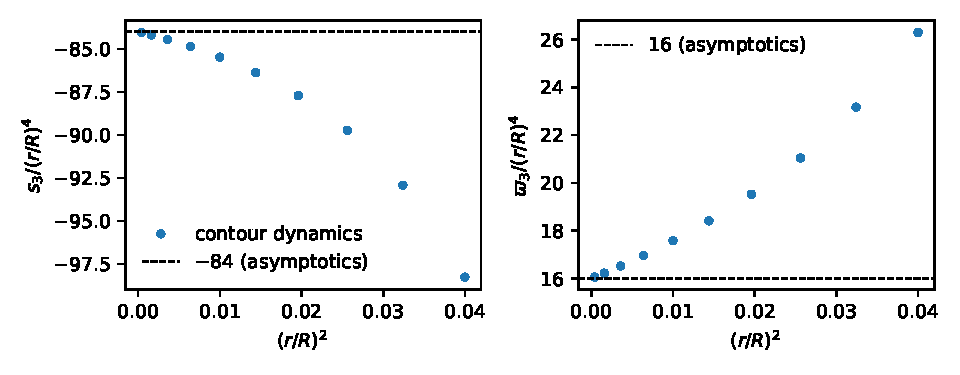
\includegraphics[width=\textwidth]{figures/fig_slowpair.pdf}
\caption{The slow $m=3$ pair of the patch heptagon from contour dynamics, $r/R\le0.2$: $s_3/(r/R)^4\to-84$ and
$\varpi_3/(r/R)^4\to16$, as in Corollary~\ref{cor:hept}.}\label{fig:slow}
\end{figure}

\subsection{The heptagon at finite core size}
\begin{result}\label{res:hept}
The steady heptagon of uniform patches is found for $0.02\le r/R\le0.28019$; continuation in $r/R$ stops there, with the smallest singular value of the Newton matrix falling to zero. For $0.02\le r/R\le0.26137$ every Bloch block has
spectrum on the imaginary axis to within $|\re\lambda|\le2\times10^{-10}$ (round-off level), so the ring is linearly stable.
At $r/R=a_c\in[0.261377,0.261379]$ (core radius over side $0.30121$; the same at $M=193$ and $M=257$) a complex quartet
appears in the Bloch blocks $m=2,5$, with $\re\lambda\approx22.7\sqrt{r/R-a_c}$. A second quartet appears in the blocks $m=1,6$ at $r/R\in[0.262194,0.262197]$ ($M=129$ and $193$;
$\re\lambda=0.29$ at $0.2624$ and $1.07$ at $0.265$).
\end{result}
\noindent\status{Numerical} \code{code/cd_heptagon_scan.py} $\to$ \code{outputs/cd_heptagon_scan.out};
\code{code/cd_onset_modes.py} $\to$ \code{outputs/cd_onset_modes.out}; \code{code/cd_onset_m1.py} $\to$
\code{outputs/cd_onset_m1.out}. Figures~\ref{fig:shapes},~\ref{fig:onset}.

\emph{Mechanism.} In the block $m=2$ we follow the eigenvalues as $r/R$ increases (Figure~\ref{fig:onset}, right). A
displacement mode, whose eigenvector has its boundary perturbation in Fourier modes $k=\pm1$, moves from $-2.58i$
($r/R=0.22$) down to $-4.4i$. An elliptical shape mode ($k=\pm2$) moves up from $-7.2i$ ($r/R=0.255$). They meet at about
$-4.88i$ at $a_c$, and leave the imaginary axis as a complex quartet. Just below $a_c$ the two modes are strongly mixed. This
is a Krein collision between a centre mode and a shape mode, which have opposite energy signatures (Lemma~\ref{lem:shape}).
It is unrelated to the order-$r^4$ mechanism of Corollary~\ref{cor:hept}: it happens when the gap between neighbouring
boundaries is about one patch radius.

\emph{End of the branch.} With $M=257$ we continue the branch to $r/R=0.28019$. The smallest singular value of the Newton matrix stays at $0.03$ up to
$0.279$ and then drops to $0.009$, and Newton's method fails beyond $0.280187$. The gap between neighbouring boundaries
there is $0.41\,r$. This points to a fold in $r/R$ at about $0.2802$; we have not
continued past it (\code{outputs/cd_onset_modes.out}).

\begin{figure}[ht]\centering
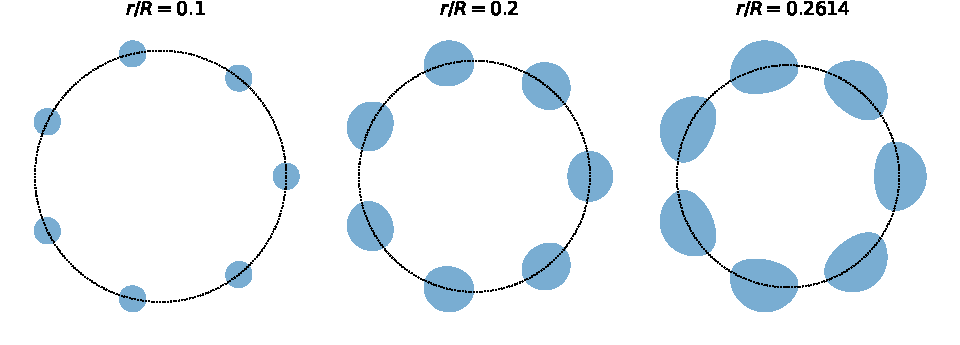
\includegraphics[width=0.9\textwidth]{figures/fig_shapes.pdf}
\caption{Steady heptagons of uniform patches (contour dynamics) at $r/R=0.1$, $0.2$ and at the onset of instability
$0.2614$.}\label{fig:shapes}
\end{figure}

\begin{figure}[ht]\centering
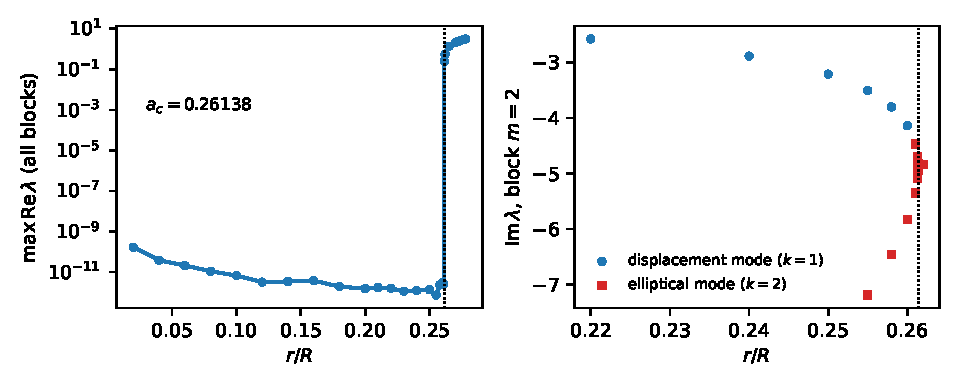
\includegraphics[width=\textwidth]{figures/fig_onset.pdf}
\caption{Left: largest real part over all Bloch blocks (after removing the trivial directions) against $r/R$; it stays at
round-off level up to $a_c=0.26138$. Right: imaginary parts of the eigenvalues of block $m=2$ in the window
$2.5<|\im\lambda|<8$. Circles mark displacement-dominated eigenvectors and squares elliptical ones; they collide at
$a_c$.}\label{fig:onset}
\end{figure}

\subsection{Independent checks by a referee}\label{sec:referee}
An independent referee wrote three further checks. We record their outputs here; they were not rerun
(\code{code/ref_cd.py}, \code{code/ref_lagr.py}, \code{code/heff_check.py}, \code{code/fitfreq.py}, unmodified;
outputs \code{outputs/ref_*.out}, \code{outputs/heff_check.out}).
\begin{itemize}
\item \emph{Linear spectrum, second code} \status{Numerical}. It uses the Cauchy form of the velocity kernel,
$u-iv=\frac{q}{4\pi}\sum_l\oint_l\frac{\bar z'-\bar z}{z'-z}\,dz'$, with the trapezoid rule, a fourth-order central
finite-difference Jacobian and Bloch blocks, at $M=65$, $97$, $129$. Its slow $m=3$ pair agrees with ours to all printed
digits, e.g.\ $0.3544572i$, $-0.4385848i$ at $r/R=0.2$, and so do the rotation rates. All blocks are stable up to $0.2613$,
and the $m=2,5$ quartet is present at $0.2615$ ($\re\lambda=0.25$), so its onset bracket is $(0.2613,0.2615)$. At $0.265$
the blocks $m=1,6$ have $\re\lambda=1.07$, as in Result~\ref{res:hept}. Its $m=0$ block shows real parts up to
$3\times10^{-4}$ at $M=97$, because that code does not quotient the rotation Jordan pair (Section~\ref{sec:spurious}).
\item \emph{Nonlinear Lagrangian contour dynamics} \status{Numerical}. Starting from the steady heptagon, the centroids are
displaced radially by $10^{-3}\cos(2\pi\cdot3k/7)$, and the full nonlinear problem is integrated with RK4 ($M=48$
Lagrangian nodes per patch, $t\le160$, about nine slow periods). The $m=3$ displacement stays bounded: its maximum is
$5.04\times10^{-4}$ in the first third of the run and $5.01\times10^{-4}$ in the last third at $r/R=0.20$, and
$5.00\times10^{-4}$ and $4.94\times10^{-4}$ at $r/R=0.15$. Its spectral peaks, at $0.355$, $-0.439$ ($r/R=0.20$) and
$0.202$, $-0.2225$ ($0.15$), match the linear eigenvalues $0.3545$, $-0.4386$ and $0.2016$, $-0.2220$. The relative patch-area
error grows to $2\times10^{-4}$ ($0.20$) and $10^{-3}$ ($0.15$), with a slow drift of the $m=0$ radial mode, which we
attribute to the coarse Lagrangian resolution.
\item \emph{The coefficients without lattice sums} \status{Numerical}. Direct 40-digit finite differences of $H_{\rm eff}$
in log-polar coordinates give, for $N=7$, $\Omega_1=-1$ and $(d^\perp,d^\parallel,d^\varpi)=(26,26,25)$, $(26,50,35)$,
$(14,56,16)$ for $m=1,2,3$, as in Theorem~\ref{thm:blocks}.
\end{itemize}

\subsection{Spurious real eigenvalues}\label{sec:spurious}
An earlier independent check with a dense finite-difference Jacobian (reviewer's code, even $M$) reported, at
$r/R=0.20$--$0.22$, a single real eigenvalue that grew with resolution; the reviewer read it as round-off in the near-zero cluster. We reran that code at $r/R=0.20$ ($M=64$, $96$) and analysed the zero cluster with our code. We did not rerun it at $0.21$ and $0.22$; with our code those points are stable (Result~\ref{res:hept}, with resolution checks at both). Real eigenvalues of this kind come from three sources, all of them
trivial directions in exact arithmetic:
\begin{enumerate}
\item For even $M$ the Nyquist mode of each boundary is invisible to the spectral derivative. It produces one spurious
eigenvalue at $0$ per Bloch block. We use odd $M$.
\item The rotation symmetry gives a $2\times2$ Jordan block at $0$ in the $m=0$ sector. A perturbation of size $\delta$ splits
it into $\pm\sqrt\delta$. With the finite-difference Jacobian ($\delta\sim10^{-9}|J|$) this gives a real pair
$\pm4.6\times10^{-4}$ (reviewer's units; $\pm0.023$ in our units) at $M=64$ and $\pm3.9\times10^{-5}$ at $M=96$
(\code{outputs/ngon_reviewer_a020.out}). With the complex-step Jacobian the split is $\le10^{-6}$ in our units. After the
quotient (ii) above it disappears.
\item The $N$ area modes (one per Bloch block) are neutral only to discretisation accuracy unless area is projected out.
\end{enumerate}
After (i)--(iii), no eigenvalue at $r/R\le0.2613$ has $|\re\lambda|>2\times10^{-10}$, at any resolution tested. The reviewer's
other findings agree with ours: the slow pair is imaginary at $r/R=0.08$ and $0.15$, with magnitudes matching
$\sqrt{84}(r/R)^2$; $N=6$ is stable; $N=8$ is unstable; and there is a strong quartet instability at $0.27$.

%======================================================================
\section{The sphere and the hyperbolic plane}\label{sec:curved}

The same construction applies to rings of patches on the unit sphere $S^2$ and the hyperbolic plane $H^2$, at height
$X_0$ ($X_0=\cos$ of the colatitude on $S^2$, $\cosh$ of the ring radius on $H^2$). Let $y=X_0^2$. In a stereographic
coordinate $z$ with metric $4|dz|^2/(1+K|z|^2)^2$ ($K=\pm1$), the same adiabatic elimination as in Proposition~\ref{prop:heff},
carried out with the conformal factor, gives the effective Hamiltonian (status \textbf{Derived}; we state the result
without repeating the derivation)
\[ H_{\rm eff}=H+r^4\sum_k\Big(\frac{1+K|z_k|^2}2\Big)^4|G_k|^2,\qquad
G_k=\frac12\sum_{l\ne k}\Big(\frac1{z_k-z_l}-\frac{K\bar z_k}{1+K|z_k|^2}\Big)^2, \]
with $H$ the point-vortex Hamiltonian of the Green function $G$ (on $H^2$, $G$ with its uniform background). We derived the
compact form of $G_k$ by hand from $f_{zz}-2\Phi_zf_z$, where $e^{2\Phi}$ is the conformal factor. For $K=0$ it reduces
to~\eqref{eq:heff}. The time-rescaling factor $\cos_K^2(r/2)$ multiplies the symplectic form and the momentum alike, and
does not move thresholds.

The same lattice-sum reduction (\code{code/blocks.py}, now with $\rho=|z|$ symbolic) gives, at the critical mode, a
stiffness $a^\perp=\frac12[(N-1)(1+y)-\floor{N^2/4}]+\epsilon\,\mathfrak A_N(y)/(1-y)^2$ with $\mathfrak A_N$ a quadratic
polynomial. The stability threshold $y=\Theta_N=\floor{N^2/4}/(N-1)-1$ moves to $\Theta_N+\mathfrak D_N\epsilon$, where
$\mathfrak D_N=-2\mathfrak A_N(\Theta_N)/[(N-1)(1-\Theta_N)^2]$ and the stable side is $y>$ threshold.

\begin{proposition}[Curved rings, $G$ model]\label{prop:curved}
For $N=4,\dots,12$ (exact rational arithmetic, \code{code/curved.py}):
\begin{center}\small
\begin{tabular}{rlll}\toprule
$N$&surface&$\mathfrak A_N(y)$&$\mathfrak D_N$\\\midrule
4&$S^2$&$-\frac{15}{16}y^2+\frac{55}{16}y-\frac98$&$+\frac18$\\
5&$S^2$&$-3y^2+\frac{27}2y-\frac{11}2$&$-1$\\
6&$S^2$&$-\frac{115}{16}y^2+\frac{1547}{36}y-\frac{230}9$&$-\frac{380}9$\\
7&--&$-\frac{27}2y^2+98y-\frac{141}2$ \ ($\mathfrak A_7(1)=14$)&no threshold off the plane\\
8&$H^2$&$-\frac{371}{16}y^2+\frac{3319}{16}y-\frac{1519}8$&$-\frac{539}4$\\
9&$H^2$&$-36y^2+\frac{3386}9y-402$&$-\frac{244}3$\\
10&$H^2$&$-\frac{855}{16}y^2+\frac{1315}2y-840$&$-\frac{2880}{49}$\\
11&$H^2$&$-75y^2+1050y-1525$&$-55$\\
12&$H^2$&$-\frac{1639}{16}y^2+\frac{236255}{144}y-\frac{197725}{72}$&$-\frac{179575}{3528}$\\\bottomrule
\end{tabular}
\end{center}
The same polynomial $\mathfrak A_N$ serves $S^2$ and $H^2$, and $\mathfrak A_N(1)$ is the planar value of
Corollary~\ref{cor:crit}. The general-$N$ forms are~\eqref{eq:curvedgeneral} below.
\end{proposition}
\noindent\status{Derived (model); Certified (exact algebra given the model)}

\emph{General $N$.} Running the same reduction with $N$ and $m$ symbolic, using the closed forms of Lemma~\ref{lem:tsums}
(valid for $N\ge4$ and $2\le m\le N-2$, which contains the critical mode), gives on both $S^2$ and $H^2$
\begin{equation}\label{eq:curvedgeneral}
\begin{aligned}
\text{even }N:\quad\mathfrak A_N(y)&=-\tfrac{(N-1)(3N^2-12N+10)}{32}y^2+\tfrac{(N-2)(9N^4+179N^3-938N^2+1492N-760)}{2304}y\\
&\qquad-\tfrac{(N-2)^2(N-1)(3N^3+6N^2-28N+40)}{2304},\\
\text{odd }N:\quad\mathfrak A_N(y)&=-\tfrac{3(N-3)(N-1)^2}{32}y^2+\tfrac{(N-1)^2(9N^3+179N^2-965N+1169)}{2304}y\\
&\qquad-\tfrac{(N-3)(N-1)^2(N^3+2N^2-11N+12)}{768},
\end{aligned}
\end{equation}
\begin{align*}
\mathfrak D_N&=\frac{(N-2)^2(N-1)(3N^4-104N^3+612N^2-1088N+640)}{288(N^2-8N+8)^2}&&(N\text{ even}),\\
\mathfrak D_N&=\frac{(N-3)(N-1)(3N^3-101N^2+509N-539)}{288(N-7)^2}&&(N\text{ odd}).
\end{align*}
Evaluated at $N=4,\dots,12$ they reproduce the per-$N$ exact results of the table above, which
\code{curved.py} computes independently (\code{outputs/curved_general.out}). \status{Certified (exact symbolic computer algebra, \code{code/curved_general.py}) given the model; not Lean}.
From them: $\mathfrak D_N<0$ for $5\le N\le27$, $N\ne7$; $\mathfrak D_4>0$; $\mathfrak D_N>0$ for $N\ge28$; and the threshold
formula, the tabulated values and $\mathfrak A_N(1)=$ Corollary~\ref{cor:crit} follow \status{Lean: \code{Heptagon.Curved},
\code{D_from_A_even}, \code{D_from_A_odd}, \code{D_values}, \code{A_at_one_even}, \code{A_at_one_odd}, \code{D_neg_small},
\code{D4_pos}, \code{DEven_pos}, \code{DOdd_pos}}.

On $S^2$, finite cores shrink the stable range for $N=4$ ($\mathfrak D_4>0$) and enlarge it for $N=5,6$. On $H^2$ the $G$ model carries a compensating uniform background vorticity. We therefore also treat the kernel
$G_1=-\log\tanh(d/2)$, with the same construction (the effective Hamiltonian has the form above with $f$ built from $G_1$).
The point-vortex ring with $G_1$ has a stability threshold $\xi_*$ in $\xi=\tanh^2(r_{\rm ring}/2)$ for $N\ge8$, and it moves to
$\xi_*+\mathfrak D^{\tanh}_N\epsilon$ with
$\mathfrak D^{\tanh}_8,\dots,\mathfrak D^{\tanh}_{12}=-26.096064,\ -13.426249,\ -8.0859592,\ -6.6885222,\ -5.3961166$. The thresholds and shifts are computed by symbolic
Taylor expansion with the Bloch substitution, as in \code{blocks.py}, with the sums over the other vortices evaluated directly
to 50 digits; the root and its derivative use double-precision secant and central differences (\code{code/tanh_check.py})
\status{Numerical, given the Derived model}. All five are negative, so the $G_1$ threshold moves to smaller rings.

%======================================================================
\section{Relation to prior work}\label{sec:prior}

\emph{Point vortices.} The linear stability of the $N$-gon is due to Thomson~\cite{Thomson1883}, with Havelock's
correction~\cite{Havelock1931}: stable for $N\le6$, neutral for $N=7$, unstable for $N\ge8$; see the review of Aref et
al.~\cite{Aref2003}. Nonlinear stability of the heptagon was proved by Cabral and Schmidt~\cite{CabralSchmidt1999} and
Kurakin and Yudovich~\cite{KurakinYudovich2002}. Proposition~\ref{prop:pv} is this classical result.

\emph{Small cores, models.} An $(r/R)^4$ correction from strain-induced elliptical deformation is standard in the
elliptical-moment model of Melander, Zabusky and Styczek~\cite{MZS1986}, and it reflects the small-strain response of
Moore and Saffman~\cite{MooreSaffman1971} and Kida~\cite{Kida1981}. Yang and Kubota~\cite{YangKubota1994} found for the
counter-rotating pair that the shape changes at order $(r/R)^2$ while the velocity changes only at a higher order; they also
report (via a private communication) that Dhanak used an expansion in $r/R$. Proposition~\ref{prop:heff} is in this tradition,
and we do not claim it as new. What we have not found in the literature is the closed form of the order-$(r/R)^4$ blocks for
all $N$ and $m$ (Theorem~\ref{thm:blocks}), the resulting value $a^\perp_3=+14(r/R)^4$ for the heptagon, and a machine check
of the algebra.

\emph{The heptagon of patches.} Here our conclusion contradicts the literature.
\begin{itemize}
\item Dhanak~\cite{Dhanak1992} (abstract; we could not obtain the full text) treated small uniform cores analytically, with
``approximate equations for the shape and motion of a vortex subjected to an external velocity field''. He found ``the
system is stable if $N<7$ and unstable if $N\ge7$'', in general agreement with Dritschel~\cite{Dritschel1985} ``except in a
region of parameter space where a high degree of accuracy is required in the numerical calculation to resolve the growth
rate of small disturbances''.
\item Polvani and Dritschel~\cite[p.~52]{PolvaniDritschel1993}: ``when $N=7$, any finite size leads to instability -- see
Dhanak 1992''.
\item Llewellyn Smith and Crowdy~\cite{LlewellynSmithCrowdy2012}: in Dritschel's study~\cite{Dritschel1985} the heptagon
``becomes unstable to a displacement instability when the point vortices are replaced by vortex patches, even very small
ones \dots\ Dhanak (1992) argues that there are, in fact, two such instabilities.'' We could not read Dritschel's paper
either.
\end{itemize}
\textbf{Contrary to the statement in Dhanak (1992), repeated in Polvani and Dritschel (1993), we find that small uniform cores
make the heptagon linearly stable.} The evidence has two independent parts: the order-$(r/R)^4$ blocks
(Theorem~\ref{thm:blocks}, given Proposition~\ref{prop:heff}), and the contour dynamics. The latter reproduces the
coefficient $-84$ to $10^{-5}$ and finds the spectrum on the imaginary axis to round-off up to $r/R=0.2614$. An independent referee's
code, a nonlinear simulation (Section~\ref{sec:referee}), and a reviewer's code agree. Since we have not read Dhanak's
paper we cannot locate the discrepancy. A reader with access might check:
(i) the order of the expansion: whether the decisive term for $N=7$ is computed at order $(r/R)^4$, and whether an
$(r/R)^2$ term appears, which would contradict Lemma~\ref{lem:newton};
(ii) the treatment of the shape. For $N=7$, $m=3$ the pieces of Proposition~\ref{prop:reduction} are $\mu=-1$,
$\Lambda_+=10$, $\Lambda_-=6$, $\kappa=22$, so
\[ d^\perp=\tfrac14(\Lambda_+^2+\Lambda_-^2)+\mu\kappa+2\mu^2=34-22+2=14,\qquad d^\parallel=34+22=56. \]
The positive part $34$ comes from the term $|L_k|^2$, i.e.\ from the ellipses \emph{following} the perturbed strain. A
model that freezes each ellipse at its equilibrium shape (shape amplitude fixed at $r^2\overline{M_k^0}$) keeps the
same rotation rate but loses exactly this term: it gives $d^\perp=-20$, $d^\parallel=22$, so $a^\perp_3a^\parallel_3<0$ and
the heptagon would be \emph{unstable}. Dropping the $|L|^2$ term for any other reason has the same effect. We verified both
numbers by direct 40-digit differentiation of the two Hamiltonians (\code{code/frozen_check.py} $\to$
\code{outputs/frozen_check.out}). This is a concrete candidate for where an approximate shape model could differ from
ours. Reversing the sign of the whole $r^4$ term would also give $-14$. The contour dynamics confirms the slaved value
(Table~\ref{tab:cd});
(iii) the definition of stability: whether ``unstable'' refers to the mode $m=3$ or to a resonance with shape modes at
finite $r$, and whether area, rotation and Jordan directions are factored out (Section~\ref{sec:spurious} shows how these
produce spurious real eigenvalues);
(iv) whether the finite-$r$ instability of Result~\ref{res:hept} (onset at core radius over side $0.301$) is what is meant.
The ``two such instabilities'' of Dhanak, as reported, may be a displacement--shape resonance of this kind.
Finally, Dhanak's abstract places his disagreement with Dritschel only ``in a region of parameter space where a high
degree of accuracy is required in the numerical calculation to resolve the growth rate of small disturbances''. This is
consistent with the scales here: the slow $m=3$ frequencies are tiny, $\sqrt{84}(r/R)^2\approx0.023$ at $r/R=0.05$ (our
units, against an orbital frequency $3$), so a weak spurious growth or decay of that size is easily produced by an
under-resolved computation. Wan~\cite{Wan1986} studied the stability of rotating vortex patches; we have not read it.

\emph{Existence.} Garc\'\i a~\cite[Thm.~1.1]{Garcia2021} proves existence of rotating patch polygons near Thomson
polygons for every $N\ge2$, including $N=7$ (Remark~\ref{rem:existence});
Hmidi--Mateu~\cite{HmidiMateu2017} and Hassainia--Wheeler~\cite{HassainiaWheeler2022} treat related multipole patch
equilibria. None of these addresses linear stability.

%======================================================================
\section{Status and limitations}

\begin{itemize}
\item \textbf{The effective Hamiltonian is formal.} Proposition~\ref{prop:heff} (adiabatic elimination of the fast
elliptical modes, remainders order-counted) is not a theorem. Consequently the stability of the small-core heptagon
(Corollary~\ref{cor:hept}) is \emph{Derived}, not proved. A proof would need a rigorous reduction of the patch dynamics
near the steady ring to a slow manifold, with error bounds of order $r^6$ in the block.
\item \textbf{Existence} of the steady patch heptagon for small patches is Garc\'\i a's theorem, which covers $N=7$
(Remark~\ref{rem:existence}); it gives boundaries at least $C^1$, and the smoothness used in our expansions is not checked
beyond that. Numerically the branch exists up to $r/R\approx0.2802$.
\item \textbf{Linear only.} We say nothing about nonlinear stability; the energy--Casimir method fails here.
\item \textbf{What Lean checks:} the lattice sums for all $N$, the block polynomials and the critical-mode signs for all $N$,
the heptagon values, the spectral criterion of a block, the algebra of the elimination, and Newton's theorem for the
logarithm on circles. \textbf{What Lean does not check:} the Taylor expansion and Bloch evaluation that turn $H_{\rm eff}$ into
lattice sums (Proposition~\ref{prop:reduction}; by hand, and cross-checked by computer algebra), the shape energy
(Lemma~\ref{lem:shape}; by hand), the adiabatic elimination itself, and all numerics.
\item \textbf{Numerics} are floating point (spectral contour dynamics). They were checked for resolution
($M=33$--$257$), against exact solutions, and against the asymptotics, but they carry no error bounds.
\item \textbf{The curved-surface coefficients} (Section~\ref{sec:curved}) depend on the curved effective Hamiltonian, which we
state without a full derivation (only the compact form of $G_k$ is derived here). They were not checked by contour dynamics here.
\item \textbf{Prior work} could not be read in full (Dhanak 1992, Dritschel 1985, Wan 1986). The conflict is reported as found.
\end{itemize}

\section*{Acknowledgement and disclosure of AI assistance}
This work was developed with substantial assistance from an AI system (Claude, Anthropic), covering the derivations, the
computer-algebra and numerical code, the Lean formalisation, and the drafting of this manuscript; the author directed the
work and takes responsibility for the content. An independent AI reviewer wrote a second contour-dynamics code used as a
cross-check. No human expert has yet checked the mathematics, and we welcome corrections, in particular from readers with
access to Dhanak (1992) and Dritschel (1985).

\appendix
\section{Proof of Proposition~\ref{prop:reduction}}\label{app:reduction}

Write $u_k=s_k+it_k$, so $z_k=\zeta^ke^{u_k}$, and $c_j=1-\zeta^j=1/p_j$. Every term of $F$ is a sum over $k$ of a local term;
by the shift symmetry, $B_m$ is obtained from the local terms at $k=0$. Write $\nabla^2_{ab}$ for the second derivatives with
respect to $(s_a,t_a)$ and $(s_b,t_b)$.

\emph{The momentum.} $J=\frac12\sum e^{2s_k}$ contributes $\partial_{s_0}J=1$, and $-\Omega\left(\begin{smallmatrix}2&0\\0&0\end{smallmatrix}\right)$ to every $B_m$.

\emph{The point-vortex energy.} For the pair $(0,j)$,
$\log(z_0-z_j)=\log c_j+\log(1+p_j\delta)$ with $\delta=(e^{u_0}-1)-\zeta^j(e^{u_j}-1)$. The quadratic part of
$\log(1+p_j\delta)$ is $\frac12p_j(u_0^2-\zeta^ju_j^2)-\frac12p_j^2(u_0-\zeta^ju_j)^2=-\frac12\zeta^jp_j^2(u_0-u_j)^2$. Here we
used $1-p_j=-\zeta^jp_j$ and $1+\zeta^jp_j=p_j$ (the coefficients of $u_0^2$, $u_j^2$, $u_0u_j$ are $-\frac12\zeta^jp_j^2$,
$-\frac12\zeta^jp_j^2$, $\zeta^jp_j^2$). Since $g_j:=\zeta^jp_j^2=-1/(4\sin^2(\pi j/N))$ is real, the quadratic part of
$H=-\sum_{k<l}\re\log(z_k-z_l)$ is $\frac12\sum_{k<l}g_{l-k}\big[(s_k-s_l)^2-(t_k-t_l)^2\big]$. Hence
$B_m(H)=\mathrm{diag}\big(g(0)-g(m),\,-(g(0)-g(m))\big)$ with $g(n)=\sum_jg_j\zeta^{jn}=T_2(n)-T_1(n)$. The linear part gives
$\partial_{s_0}H=-\re\sum_jp_j=-\frac{N-1}2$, so $\Omega_0=-\frac{N-1}2$ and $-2\Omega_0=N-1$.

\emph{The core term.} Let $m_k=\zeta^{2k}M_k=\sum_{j\ne0}(e^{u_k}-\zeta^je^{u_{k+j}})^{-2}$, so $|m_k|=|M_k|$. Expanding
$(c_j+\delta)^{-2}=p_j^2(1-2p_j\delta+3p_j^2\delta^2-\dots)$ gives $m_k=\mu+L_k+q_k+O(u^3)$, with $\mu=T_2(0)$ real,
\[ L_k=\sum_l\lambda_{l-k}u_l,\quad\lambda_0=-2\sum_jp_j^3,\ \lambda_j=2\zeta^jp_j^3\ (j\ne0),\qquad
q_k=\sum_j\big[-p_j^3(u_k^2-\zeta^ju_{k+j}^2)+3p_j^4(u_k-\zeta^ju_{k+j})^2\big]. \]
Then $|m_k|^2=\mu^2+2\mu\re L_k+|L_k|^2+2\mu\re q_k+O(u^3)$. Set $\Lambda(n)=\sum_j\lambda_j\zeta^{nj}=-2(T_3(0)-T_3(n+1))$.
It is real, because $\lambda_{-j}=\bar\lambda_j$. For $|L|^2=\sum_k L_k\bar L_k$ we have
$\partial_{s_a}\partial_{s_b}=\partial_{t_a}\partial_{t_b}=2\re\sum_k\lambda_{a-k}\bar\lambda_{b-k}$ and $\partial_{s_a}\partial_{t_b}=2\im\sum_k\lambda_{a-k}\bar\lambda_{b-k}$. Summing against $\zeta^{mb}$ gives the block
contributions $\Lambda(m)^2+\Lambda(-m)^2$ on the diagonal and $i(\Lambda(m)^2-\Lambda(-m)^2)$ off the diagonal. For
$\re q=\re\sum_{a,b}K_{ab}u_au_b$, with $K$ real and symmetric by the reflection symmetry, the contributions are
$\pm2\kappa$ on the diagonal ($+$ for $ss$, $-$ for $tt$) and $0$ off it. Here
$\kappa=\sum_bK_{0b}\zeta^{mb}$ is $q_0$ evaluated bilinearly on $(u_a)=(\zeta^{-ma})$, $(u_b)=(\zeta^{mb})$:
\[ \kappa=\sum_j\big[-p_j^3(1-\zeta^j)+3p_j^4(1-\zeta^{j(1-m)})(1-\zeta^{j(1+m)})\big]
=-T_2(0)+3\big(T_4(0)-T_4(1-m)-T_4(1+m)+T_4(2)\big). \]
Multiplying by $\frac14$ (from $\Phi=\frac14\sum|m_k|^2$) and by $2\mu$ where appropriate gives the bracketed terms. Finally,
$\partial_{s_0}\Phi=\frac12\mu\Lambda(0)=-\mu T_2(0)=-\mu^2$ (by Lemma~\ref{lem:tsums}(b)), so $\Omega_1=-\mu^2$ and $-2\Omega_1=2\mu^2$. $\square$

\section{Numerical details}\label{app:num}
Steady states are converged to residual $\le2\times10^{-12}$; the smallest singular value of the Newton matrix stays
$\ge0.03$ for $r/R\ge0.2$. The resolution schedule is $M=65$ for $r/R\le0.205$, $129$ up to $0.255$, and $193$ beyond, with
checks at $129$, $193$ and $257$; the branch continuation beyond $0.278$ uses $M=257$ with the step refined down to $10^{-5}$. The onset was bisected to width $2\times10^{-6}$ at $M=193$ and $M=257$ with the
criterion $\max\re\lambda>10^{-7}$. Run times are minutes per point on a workstation; \code{run_all.sh} with the option \code{--fast} reproduces a
reduced set.

\bibliographystyle{plain}
\bibliography{refs}
\end{document}
